\part{Demokratie und Diktatur -- Anspruch und Wirklichkeit von
Gesellschaftsmodellen in der ersten Hälfte des 20. Jahrhunderts}
\label{prt:dem-dikt}

\chapter{Das Deutsche Reich 1919 bis 1933 -- Die Weimarer Republik}
\label{chp:weim-rep}
\index{Deutsches Reich!1919 bis 1933}
\index{Weimarer Republik}

\begin{aufgabe}
Erläutern Sie den Platz der Weimaerer Republik in der deutschen
Geschichte!

Weisen Sie diese Position an der Weimarer Verfassung nach!
\end{aufgabe}

\section{Der \ins{Vertrag von Versailles}}
\label{sec:vvv}
\index{Erster Weltkrieg}
\index{Friedensvertrag!Versailles}

Die Verhandlungen über den Friedensvertrag der Alliierten des Ersten
Weltkrieges mit Deutschland \ort{begannen im Januar 1919}
\ort{Versailles}. Die Bedingungen wurden am \dat{23. Juni 1919} an die
deutsche Delegation, die an den vorangehenden Zusammenkünften nicht
teilnehmen durfte, übergeben und am \dat{28. Juni} im Spiegelsaal
\index{Spiegelsaal} von Versailles unterzeichnet.

\subsection*{Gebietsregelungen}

\begin{itemize}
\item \ort{Elsaß-Lothringen} geht an Frankreich.
\item \ort{Westpreußen} geht an Polen.
\item Schaffung eines polnischen Korridors zur Ostsee
\item \ort{Danzig} wird freie Stadt; Polen erhält Sonderrechte im
Hafen von Danzig
\item Das \ort{Memelgebiet} geht an Litauen, später an die
Sowjetunion.
\item \ort{Eupen-Malmedy} geht an Belgien.
\item Das \ort{Saargebiet} wird dem \ins{Völkerbund} unterstellt.
\item Die \ins{Saargruben} gehen zur Ausbeutung 15 Jahre an
Frankreich.
\item Die deutschen Kolonien\index{Kolonien!deutsch} werden dem
Völkerbund unterstellt.
\end{itemize}

\noindent $\Longrightarrow$ Deutschland verliert 10\,\% seiner
Bevölkerung und 13\,\% seiner Fläche


\subsection*{Politische Regelungen}

\begin{itemize}
\item Verbot eines Zusammenschluss des Deutschen Reiches mit
Österreich (eigentlich durch den \ges{Vertrag von Saint
Germain}\Ort{Saint Germain}{}
\item Das Deutsche Reich erhält mit dem §\,231 die alleinige
Kriegsschuld und daraus abgeleitet die Pflicht zur Zahlung aller
Reparationen. \index{Kriegsschuldparagraph}\index{Reparationen!Erster
Weltkrieg} 
\end{itemize}


\subsection*{Militärische Regelungen}

\begin{itemize}
\item Reduzierung der deutschen Armee auf 100\,000 Mann, der Marine
auf 15\,000 Mann.
\item Verbot von Flugzeugen, Panzern, U-Booten und schweren
Kriegsschiffen
\item Auslieferung der Kriegsflotte
\item Verbot eines Generalstabes\index{Generalstab}
\item militärische Besetzung des linken \Ort{Rheinufer}{Rheinufers}
durch Frankreich, einige rechtsrheinische
Brückenköpfe\index{Rheinufer!Brückenköpfe} für 15 Jahre
\item Entmilitarisierung eines rheinischen Streifens
\end{itemize}


\subsection*{Wirtschaftliche Regelungen}

\begin{itemize}
\item durch die Gebietsabtrennungen betroffen: Bergbau,
Stahlindustrie, Hüttenwesen, Landwirtschaft
\item \dat{1921 Fixierung} der Reparationen auf 132 Milliarden
Reichsmark\index{Reparationen!Erster Weltkrieg}
\end{itemize}


\subsection*{Folgen in Deutschland}

\begin{itemize}
\item Austritt der \ins{DDP} aus der \ort{Weimarer Koalition}

\item Rücktritt des Ministerpräsidenten \Nam{Scheidemann,
Philipp!Rücktritt}{Scheidemann} und des Außenministers
\Nam{Brockdorff-Rantzau, Ulrich von!Rücktritt}{von Brockdorff-Rantzau}

\item gleichfalls Rücktritt des Reichswehrministers \Nam{Noske,
Gustav!Rücktritt}{Noske} (\ins{SPD}) und des verfassungstreuen Generals
und Chefs der \ins{Heeresleitung} \Nam{Reinhardt,
Walther!Rücktritt}{Reinhardt} -- Neubesetzung der Stellen durch den
\beg{Vernunftrepublikaner} \Nam{Gessler, Otto}{Gessler} (DDP) und den
Antirepublikaner General \Nam{Seeckt, Hans von}{von Seeckt}

\item Hohe Reparationszahlungen bremsen den Wiederaufbau und führen zu
Unzufriedenheit, Armut und Arbeitslosigkeit. Die übertriebenen
Ansprüche der Alliierten führen schließlich zum
\emph{Ruhrkampf}\index{Ruhrkampf} (siehe \ref{sec:krisj-1923}).
\end{itemize}



\endinput

\section{Parteien}
\mar{Siehe hierzu auch das Arbeitsblatt aus der Sekundarstufe \Rm{1}}

\subsection*{Republiksgründung}

Tabelle \ref{tab:vergl-part-weimrep} bietet eine Übersicht über die
Parteien, die bei der Gründung der Weimarer Republik bestimmend waren.
Dabei ist noch zu bemerken, dass nur SPD, DDP und Zentrum
staatstragende Parteien waren, alle Parteien eine Revision des
\ges{Vertrag von Versailles}{Vertrages von Versailles} anstrebten und
dass die DNVP den Wiedererwerb von Kolonien und die Erneuerung des
deutschen Kaisertums befürwortete.

%{
%\small
%\renewcommand{\arraystretch}{0.8}
%
%% Wir müssen doch mal wieder berechnen.
%\newlength{\frstcolwdth}
%\settowidth{\frstcolwdth}{\textit{Zentrum}}
%
%\newlength{\dumwdth}
%\setlength{\dumwdth}{\textwidth}
%\addtolength{\dumwdth}{-\frstcolwdth}
%\newlength{\othcolwdth}
%\setlength{\othcolwdth}{0.5\dumwdth}
%\addtolength{\othcolwdth}{-3\tabcolsep}
%
%\tablecaption{bla}
%\tablefirsthead{
%\toprule
%
%Partei &
%Politisches System &
%Wirtschaftliches System \\
%
%\midrule
%}
%
%\begin{supertabular*}{\textwidth}{cp{\othcolwdth}p{\othcolwdth}}
\begin{table}
\caption{Vergleich von Parteien der Weimarer Republik}
\label{tab:vergl-part-weimrep}

\renewcommand{\arraystretch}{0.8}
\footnotesize

\begin{tabularx}{\textwidth}{cXX}
\toprule

Partei &
Politisches System &
Wirtschaftliches System \\

\midrule

\Ins{DNVP, Deutschnationale Volkspartei}{DNVP} &
\vspace{-0.7em}
\begin{tablist}
\item überparteiliche (Hohenzollern-) Monarchie 
\item starke Exekutive
\item Mitwirkung des Parlaments bei der Gesetzgebung
\item Ständevertretung zusätzlich zur Volksvertretung
\end{tablist}
&
\vspace{-0.7em}
\begin{tablist}
\item Eigenwirtschaft und Privateigentum
\item Sozialisierung mit äußerster Vorsicht
\item Förderung eines starken Mittelstandes und der Landwirtschaft 
\end{tablist}
\\

\Ins{DVP, Deutsche Volkspartei}{DVP} &
\vspace{-0.7em}
\begin{tablist}
\item Monarchie
\item Verantwortliche Mitwirkung des Parlaments an der Regierung 
\end{tablist}
&
\vspace{-0.7em}
\begin{tablist}
\item Privatwirtschaft
\item keine Sozialisierung
\item Förderung der Landwirtschaft und des Mittelstandes 
\end{tablist}
\\

\Ins{DDP, Deutsche Demokratische Partei}{DDP} &
\vspace{-0.7em}
\begin{tablist}
\item demokratische Republik auf dem Boden der Weimarer Verfassung
\item liberaler und sozialer Rechtsstaat 
\end{tablist}
&
\vspace{-0.7em}
\begin{tablist}
\item Privatwirtschaft
\item gegen jegliche Vergesellschaftung
\item Schutz von Handwerk und Mittelstand 
\end{tablist}
\\

\Ins{Zentrum, Deutsche Zentrumspartei}{Zentrum} &
\vspace{-0.7em}
\begin{tablist}
\item demokratische Republik 
\item christliche Grundsätze
\item bürgerliche Freiheiten
\item soziale Gerechtigkeit
\end{tablist}
&
\vspace{-0.7em}
\begin{tablist}
\item Recht auf Privateigentum
\item Förderung des Genossenschaftswesens
\item Verstaatlichung nur gegen Entschädigung
\item Schutz des Mittelstands und des Bauernstands
\end{tablist}
\\

\Ins{SPD, Sozialdemokratische Partei Deutschlands!Weimarer
Republik}{SPD} &
\vspace{-0.7em}
\begin{tablist}
\item demokratische Republik
\item Demokratisierung des Staates und der Gesellschaft
\item Erneuerung der Gesellschaft
\item sozialistisches Gemeinwesen
\end{tablist}
&
\vspace{-0.77em}
\begin{tablist}
\item Überwindung des kapitalistischen Systems
\item Förderung des gemeinwirtschaftlichen Gedankens
\item Genossenschaftswesen
\item Überführung der Konzerne in die GemeInschaft
\item Verstaatlichung von Grund und Boden
\end{tablist} 
\\

\Ins{KPD, Kommunistische Partei Deutschlands!Weimarer Republik}{KPD} &
\vspace{-0.7em}
\begin{tablist}
\item Errichtung einer sozialistischen Gesellschaftsordnung
\item revolutionäre Umgestaltung von Staat, Gesellschaft und
Wirtschaft
\item Übernahme der staatlichen Funktionen durch Arbeiterräte 
(Räterepublik)
\end{tablist}
&
\vspace{-0.7em}
\begin{tablist}
\item Enteignung von Banken, Industrie --
Vergesellschaftung der Industrie und des Kapitals
\item Enteignung von Großgrundbesitz -- Bildung sozialistischer
landwirtschaftlicher Genossenschaften
\end{tablist}
\\

\bottomrule
\end{tabularx}
\end{table}
%\end{supertabular*}
%}

\subsection*{Rechtsextremistische Strömung}
\index{Antimarxismus}
\index{Antiliberalismus}
\index{Antisemitismus}
\index{Jugendkult}
\index{Führerkult}
\index{Nationalsozialismus!Weimarer Republik}

Zu Anfang der Weimarer Republik noch von geringer Bedeutung, nahm die
Bedeutung der rechtsextremistische Strömung, politisch vor allem durch
die \ins{NSDAP, Nationalsozialistische Deutsche Arbeiterpartei}{NSDAP}
verkörpert, rasch zu. Sie war charakterisiert durch ideologische
Prägung mit \emph{Antimarxismus}, \emph{Antiliberalismus} und
\emph{Antisemitismus}, Betonung von Werten wie Einigkeit und Treue,
Militarismus als Lebenform und völkisch mystifizierten Jugend- und
Führerkult.

Mit den Konservativen gemein hatten sie die starke Ablehnung der
Weimarer Republik (\jar{Republik der Novemberverbrecher}) und die
Forderung nach einem starken Staat. Sie zeichneten sich aber durch
größere Radikalität, die auch vor Gewalttaten bis hin zu Morden nicht
zurückschreckte, Bildung einer \jar{kriegerischen Elite} sowie das
Ziel eines \jar{nationalen Sozialismus} aus.

\endinput

\section[Revisions- und Erfüllungspolitik -- Die Rolle politischer
Handlungsträger]{Revisions- und Erfüllungspolitik -- Die Rolle
politischer
Handlungsträger\mycite[339\,--\,348]{braunesGeschichts}\,\mycite[356\,--\,360]{gelbesGeschichts}\,\mycite[26\,f.,
32\,f.]{IzpBWeimRep}}
\label{sec:rev-erf-pol}
\index{Revisionspolitik}
\index{Erfüllungspolitik}

\subsection*{Vertrag von Rapallo}

Nach dem Ersten Weltkrieg standen die Russische Sozialistische
Föderative Sowjetrepublik (RSFSR) und das Deutsche Reich
wirtschaftlich und politisch isoliert da. -- Erstere wegen der
westlichen Angst vor dem Kommunismus, letzteres wegen seiner Rolle im
Krieg. In dieser Situation beschlossen sie \dat{1922 im \ges{Vertrag
von Rapallo}} gegenseitigen \Ort{}{Rapallo}
\emph{Reparationsverzicht}\index{Reparationen!Rapallo}, Aufnahme
\emph{diplomatischer Beziehungen} und
\emph{Meistbegünstigung}\index{Meistbegünstigung!Rapallo} in den
wirtschaftlichen Beziehungen. Gleichzeitig wurde der \ges{Vertrag von
Versailles} unterwandert, indem die Hilfe deutscher Experten bei der
Entwicklung russischen schweren Kriegsgeräts vereinbart wurde, was mit
der Möglichkeit der Übung deutscher Militärs am Material einherging.

Der Vertrag von Rapallo verärgerte also durch die Veränderung der
Situation in Osteuropa Großbritannien und Frankreich und übte
gleichzeitig Druck auf diese aus. Denn nun waren Polen und die
Tschechoslowakei, die eine Schutzgürtel gegen den Kommunismus bilden
sollten, in eine Zweifrontenlage geraten. Es war nun die Zeit für
Deutschland gekommen, außenpolitisch aktiv zu werden.

%%%%%%%%%%%%%%%%%%%%%%%%%%%%%%%%%%%%%%%%%%%%%%%%%%%%%%%%%%%%%%%%%%%%%%

\subsection*{Ära Stresemann}
\index{Ära Stresemann}

\nam{Stresemann, Gustav}{Gustav Stresemann} war von August bis
November 1923 Reichskanzler und danach bis zum seinem Tode im Jahre
1929 Außenminister in der Weimarer Republik. Seine Rolle in der
Politik der damaligen Zeit war bestimmen, weswegen man von der
\jar{Ära Stresemann} spricht, sodass sein Ableben zu einem Machtvakuum
führte, das in die Präsidialkabinette (siehe \ref{sec:praes-kab})
mündete.

Seine Ziele war das Wiedererstarken Deutschlands auf Grundlage der
Lösung des Reparationsproblems und der Revision des \Ges{Vertrag von
Versailles}{Vertrags von Versailles}, die mit der Korrektur der
Ostgrenzen, der Vereinigung mit Deutsch-Österreich und dem Schutz der
Auslandsdeutschen einhergingen. Er war also eindeutig ein
Revisionspolitiker, sah aber anders als viele andere Gegner des
Vertrags von Versailles die einzige Möglichkeit der Erreichung seiner
Ziele in der Friedenssicherung durch die Aussöhnung mit Frankreich und
den Eintritt in den \ins{Völkerbund}.\mycite{StresWil}

\subsubsection{Dawes-Plan}
\index{Dawes-Plan}

Da das Deutsche Reich offensichtlich Schwierigkeiten hatte
(\emph{Ruhrkampf}\index{Ruhrkampf}, siehe \ref{sec:krisj-1923}),
seinen Reparationspflichten nachzukommen, legte der US-amerikanische
Bankier \nam{Dawes, Charles}{Charles Dawes} ein Programm vor, dass
einen angemessenen Zahlungsplan sowie die Möglichkeit der
Kreditaufnahme vorsah. Dabei wollten die USA gleichfalls Absatzmärkte
schaffen -- das Geld aus dem Kredit über 800 Millionen Reichsmark
musste in den USA ausgegeben werden -- und den internationalen Markt
stabilisieren, um die Gefahr der Ausbreitung des Kommunismus mindern.

\dat{1924 unterzeichneten} die beteiligten Mächte auf der
\ins{Londoner Konferenz}\Ort{London}{} das betreffende Abkommen,
welches zugleich zur wirtschaftlichen und politischen internationalen
Integration des Deutschen Reiches (\emph{Eintrittskarte} nach Europa)
und damit zur Entspannung in Europa führte. Die ökonomische
Stabilisierung in Deutschlands war auch Ursache für die Scheinblüte der
\jar{Goldenen Zwanziger}.\index{Goldene Zwanziger}\index{Scheinblüte}
Allerdings war das Deutsche Reich nun finanziell von den USA abhängig.
Daher schlug die \ins{Weltwirtschaftskrise} 1929 hier besonders hart
zu.


\subsubsection{Verträge von Locarno}

Die \ges{Verträge von Locarno}\Ort{Locarno}{} wurden \dat{1925} auf
einer Konferenz von Politikern Belgiens, Deutschlands, Frankreichs,
Großbritanniens, Italiens, Polens und der Tschechoslowakei
\dat{geschlossen} und errichteten den Prinzipien der \Nam{Stresemann,
Gustav}{stresemann}schen Außenpolitik folgend ein europäisches
Sicherheitssystem.

\paragraph{Inhalte} Mit dem \ges{Westpakt} verzichteten Belgien, das
Deutsche Reich und Frankreich auf eine gewaltsame Veränderung der
gemeinsamen Grenzen.  Letzteres schloss damit auch Ansprüche auf
\ort{Eupen-Malmedy} und \ort{Elsaß-Lothringen}. Die Einhaltung dieses
Vertrages überwachten Großbritannien und Italien als Garantiemächte.

Der \ges{Rheinpakt} vereinbarte den schrittweisen Abzug der
französischen Truppen aus dem \ort{Rheinland}.

Stresemann wollte ausdrücklich keine Garantie der deutschn Ostgrenze.
Der \ges{Ostpakt} war deshalb lediglich ein Schiedsvertrag mit Polen,
der eine gewaltsame Veränderung der Grenze ausschloss.

\paragraph{Folgen} International bedeuteten die Verträge einen großen
weiteren Schritt zur Rehabilitation des Deutschen Reiches und beendete
seine außenpolitische Isolation endgültig. Sie ermöglichten nämlich
dessen \dat{Aufnahme in den \ins{Völkerbund} 1926} -- ein lange
verfolgtes Ziel Stresemanns. Hier war das Deutsche Reich ein
gleichberechtigter Partner zwischen den anderen Großmächten und hier
konnte der Außenminister der Welt seine Anliegen, insbesondere
bezüglich der Auslandsdeutschen\index{Auslandsdeutsche} vorzutragen.

National wurden die Verträge von rechts und links angefeindet. Jene
beschimpften das Vorgehen Stresemanns und der anderen Beteiligten als
\emph{Erfüllungspolitik}\index{Erfüllungspolitik}, als Schwäche und
\jar{Unehre} des Deutschen Reiches. Diese wetterten ob der angeblichen
\jar{imperialistischen} und \jar{antikommunistischen} Bestrebungen. So
oder so wurden die Verträge von Locarno eine Plattform für Propaganda
gegen die Weimarer Republik.


\subsubsection{Berliner Vertrag}

Wegen der Einbindung des Deutschen Reiches in das westliche
Staatensystem infolge der \ges{Verträge von Locarno}\Ort{Locarno}{}
befürchtete man in der UdSSR, dass sich jenes von den Festlegungen des
\Ges{Vertrag von Rapallo}{Vertrages von Rapallo}\Ort{Rapallo}{}
entfernen könnte.  Deshalb schlossen beide Staaten \dat{1926 den
\ges{Berliner Vertrag}}, indem sie sich die gegenseitige Neutralität
für den Fall eines Krieges zusicherten. Laut \cite[33]{IzpBWeimRep}
bedeutete das insbesondere, dass das Deutsche Reich den Durchmarsch
französischer Truppen bei einem Krieg zwischen der Sowjetunion und
Polen untersagen würde.


\subsubsection{Briand-Kellog-Pakt}

\dat{1928 initiierten} der französische Außenminister \Nam{Briand,
Aristide}{Aristide Briand}, der schon maßgeblich zum Zustandekommen
der \ges{Verträge von Locarno}\Ort{Locarno}{} beigetragen hatte, und
\Nam{Kellogg, Frank Billings}{Frank Billings Kellogg} einen
Vertrag zur Ächtung des Krieges, den \ges{Briand-Kellogg-Pakt}. Unter
den anfänglich 15 Unterzeichnerstaaten befand sich auch das Deutsche
Reich. Nach und nach traten dann weitere Staaten bei, sodass es
schließlich circa 60 wahren.


\subsubsection{Young-Plan}

Die nach wie vor nich gelöste Frage der deutschen Reparationen trieb
die Politiker weiter um, bis schließlich \dat{1929} ein unter der
Leitung des amerikanischen Wirtschaftsfachmann \Nam{Young, Owen}{Owen
Young} ausgearbeiteter Plan \ges{Young-Plan}{} \dat{verabschiedet}
wurde, der folgende Regelungen enthielt:

\begin{enumerate}
\item Die Gesamtsumme der Reparationen wird auf 114 Milliarden
Goldmark festgesetzt.
\item Deutschland soll 59 Jahre lang zahlen.
\item Die Höhe der Raten steigt in den ersten 37 Jahren von 1,7 auf
2,1 Milliarden Goldmark.
\item Ausländische Wirtschaftskontrollen in Deutschland entfallen.
\item Die alliierten Besatzungstruppen werden bereits 1930, also fünf
Jahre früher, aus Deutschland (\ort{Rheinland}) abgezogen.
\end{enumerate}

\mar{Tauch Lausanne irgendwann mit auf?}

\subsection*{Bilanz}\mar{Nur der Form halber.}

\begin{itemize}
\item Deutschland ist rehabilitiert, aber noch nicht vollständig
souverän. 
\item Der \ges{Vertrag von Versailles} (Kriegsschuldparagraph!) ist
nicht revidiert.
\item Die Verträge, insbesondere die von Locarno, bieten eine
Propagandaplattform für Republikfeinde.
\item Der \dat{Tod Stresemanns 1929} hinterlässt ein Machvakuum,
infolgedessen die Zeit der Präsidialkabinette beginnt.
\end{itemize}


\endinput

\section{Das Krisenjahr 1923}
\label{sec:krisj-1923}

Siehe hierzu das Arbeitsblatt, von dessen Autorinnen ich \Nam{Barth,
Lina}{Lina Barth} ich noch im Gedächtnis habe.

\endinput

\section{Inflation}
\label{sec:soz-veraend}
\index{Inflation!Weimarer Republik}
\index{Hyperinflation}

Während des Krieges hatte die Inflationsrate im Deutschen Reich zu
steigen begonnen. Diese Tendenz kuliminierte \dat{1923}, als die
schleichende Inflation zur galoppierenden und schließlich zur
\dat{Hyperinflation} wurde. Nun erst wurde das Problem mit der
\dat{Währungsreform vom 15. November 1923}, die die \ins{Rentenmark}
einführte, wobei eine Rentenmark den Wert von 1\,000\,000\,000\,000 (1
Bio.) Papiermark und 4,2 Dollar den Wert einer Rentenmark
hatte.\mycite[28]{IzpBWeimRep}

\subsection*{Folgen}

\subsubsection{Wirtschaft}

\begin{itemize}
\item materielle Verluste
\item Vermögensumschichtung
\item Löhne auf Vorkriegsnieveau
\item Vernichtung von Geldvermögen
\item Konzentrationsprozesse -- Konternbildung 
\end{itemize}


\subsubsection{Bevölkerung}

\begin{itemize}
\item Abhängigkeit von der Armenfürsorge
\item Zerfall des klassischen Bildungsbürgertums als Träger der
Gesellschaft durch finanzielle Entmachtung
\item Sachwertbesitzer werden zu Geldwertbesitzern
\item materielle und damit seelische Not
\item soziale Schichtung (Klassengesellschaft im Übergang)\mar{?}
\item Neuerungen im sozialen Bereich (bspw. Sozialverischerung) 
\item hohe Arbeitslosenrate
\end{itemize}


\subsubsection{Politik}

Die Inflation wirkte sich auf die Politik insofern aus, als die
Radikalisierung, das heißt die Entfernung von den Parteien der Mitte,
vorangetrieben wurde. Dies zeigte sich in den Wahlen von 1924.


\subsection*{Bilanz}

\subsubsection{Gewinner}

\begin{itemize}
\item Staat -- Lösung des Schuldenproblems
\item Sachwertbesitzer
\item Unternehmer -- Kredite aus getätigten Modernisierungs- oder
Erweiterungsinvestitionen konnten mühelos getilgt werden. 
\end{itemize}

\subsubsection{Verlierer}

\begin{itemize}
\item Staat -- Die Menschen schoben die Schuld am Elend den
staatstragenen Parteien zu und wendeten sich an die Radikalen.
\item Mittelschicht, Stadtbewohner -- Verlust von Erspartem
(Alterssicherung), großen Einkommensverluste vor der Reform
\item Ausland -- Gesamtverluste auf deutschen Bankguthaben und
Wertpapierbeständen von circa 15 Milliarden Goldmark
\end{itemize}

\endinput

\section{Jugend}

\ges{Dawes-Plan} (siehe \ref{sec:rev-erf-pol}) und
Inflation\index{Inflation} (siehe \ref{sec:soz-veraend})
bewirkten

\begin{itemize}
\item sozial:

\begin{itemize}
\item Jugendarbeitslosigkeit -- Jugendliche fallen den Familien länger
zur Last
\item Verbitterung durch fehlende Freizeitangebote:

\begin{itemize}
\item verstärkte Neigung zu Protest- und Gewalttaten 
\item Verlust der Autorität der Familie
\item Jugendkriminalität
\end{itemize}

\item \jar{vergreiste Republik} -- Die Jugend fühlt sich um Lebens-
und Karrierechancen betrogen.
\end{itemize}

\item politisch:

\begin{itemize}
\item hohe Anfälligkeit gegenüber radikalen Ideologien und
Gruppierungen
\item studentische Wahlen Ender der 1920er\mar{?} -- hoher
Stimmenanteil für völkisch-nationalistische Gruppen
\end{itemize}
\end{itemize}

Insgesamt fallen also auf:

\begin{itemize}
\item antidemokratisches Denken
\item starker Widerwille gegen westlich-liberale Weltreaktion \mar{?}
-- Radikalismus nach links und rechts
\item glauben an Ideen, statt an aufgeklärten Verstand
\end{itemize}

\endinput

\section{Auswirkungen der Weltwirtschaftskrise auf Deutschland}
\index{Weltwirtschaftskrise}
\index{Börsenkrach}
\index{Schwarzer Freitag}

Der Konjunkturrückgang in den USA führte dort am \dat{25. Oktober
1929}, dem sogenannten \emph{Schwarzen Freitag}, schließlich zum
\dat{Börsenkrach}. Infolgedessen zogen die USA die kurzfristigen
Kredite aus Deutschland (und den anderen europäischen Staaten) ab, was
dort zu Geldverknappung und Zahlungsschwierigkeiten bei den Banken
führte. Um einen vollständigen Zusammenbruch zu verhindern, trat der
Staat zwar mit Geldreserven ein. Doch der Kaufkraftverlust führte zur
Überproduktion, welche die Betriebe zu Produktionseinschränkungen
veranlasste. Diese mündeten in Massenentlassungen, sodass schließlich
die Wirtschaft völlig am Boden war. 

\endinput

\section{Präsidialkabinette}
\label{sec:praes-kab}

Siehe hierzu das altbewährte Schema und die ebenso altbewährte
Tabelle.

\endinput

\section{Gründe des Scheiterns der Weimarer Republik -- Eine Bilanz}

\begin{aufgabe}
Erarbeiten Sie aus der Quelle die Ursachen des Scheiterns der Weimarer
Republik aus Sicht des Autors!

Erläutern Sie an zwei selbst gewählten historischen Beispielen deren
destruktive Wirkung auf die Weimarer Republik!

Bewerten Sie den Stellenwert der gewählten Beispiele im Gesamtgefüge!
\end{aufgabe}

Siehe hierzu das gleichnamige Arbeitsblatt.

\endinput


\chapter{Das Deutsche Reich 1933 bis 1945}
\label{chp:drittes-reich}
\index{Deutsches Reich!1933 bis 1945}
\index{Drittes Reich}

\section{Grundlagen}

\subsection[Ideologie des
Nationalsozialismus]{Ideologie\mycite[386\,--\,389]{gelbesGeschichts}
des Nationalsozialismus}
\index{Ideologie!Nationalsozialismus}
\index{Blut und Boden}
\index{Chauvinismus}
\index{Militarismus}

{
\small
\newlength{\antsemlength}
\settowidth{\antsemlength}{Antisemitismus}

\newcommand*{\nodebox}[1]{\parbox{\antsemlength}{#1}}

\begin{bundle}{\textbf{Sozialdarwinismus}}
  \chunk[\footnotesize Blut]{\nodebox{Rassismus\newline Antisemitismus}}
  \chunk[\footnotesize Boden]{
    \begin{bundle}{\nodebox{Nationalismus\newline \beg{Chauvinismus}}}
      \chunk{Führerprinzip}
      \chunk{Lebensraumtheorie}
      \chunk{Volksgemeinschaft}
      \chunk{Militarismus}
    \end{bundle}
  }
\end{bundle}
}


\subsubsection[Rassismus und Antisemitismus]{Rassismus und
Antisemitismus (siehe auch \ref{sec:aussch-gegner})}
\index{Rassismus}
\index{Antisemitismus}
\index{Rassenantisemitismus}
\index{Rassenlehre}
\index{Arier}

\begin{itemize}
\item Biologisierung des Sozialen -- Bestimmung des Verhaltens durch
Gene
\begin{itemize}
\item Höher-/Minderwertigkeit von Rassen: \jar{arische Rasse}
(nordisch), \jar{Kuli- und Fellachenrassen} (afrikanisch und
asiatisch), Juden
\item Schwache und Bedürftige schwächen mit ihren \jar{Erbanlagen} das
\jar{deutsche Volk}
\end{itemize}

\item Antisemitismus nicht mehr aus sozialen und religiösen Gründen,
sondern Rassenantisemitismus -- \jar{jüdische Rasse} als
\jar{minderwertig} und \jar{schmarotzend}

\item Rassismus und Antisemitismus werden zum Mittelpunkt des
politischen Denkens
\end{itemize}


\subsubsection{Führerkult}
\index{Führer}
\index{Führerkult}
\index{Führerprinzip}

\begin{itemize}
\item bedingungslose Unterwerfung des Einzelnen unter die Ziele des
Staates
\item Ausschluss von Opposition
\item Vereinigung aller Gewalten im \jar{Führer} 
\end{itemize}


\subsubsection{Lebensraumtheorie/-politik}
\index{Lebensraumtheorie}
\index{Lebensraumpolitik}

\begin{itemize}
\item \jar{germanische Rasse} hat Herrschaftsanspruch
\item Ausdehnung in Richtung Osten
\item Unterwerfung der \jar{Untermenschen}
\end{itemize}


\subsubsection{Volksgemeinschaftsideologie}
\index{Volksgemeinschaft}

\begin{itemize}
\item Wiedergeburt des deutschen Reiches
\item Verbot aller Parteien außer der NSDAP
\item Zusammenfassung aller politischen und sozialen Gruppen zu einer
\jar{Volksgemeinschaft}, Unterordnung und den Willen des \jar{Führers}
-- Überwindung sozialer, beruflicher und ideologischer Unterschiede
\end{itemize}


\subsection{Sicht des Großteils der Bevölkerung auf die Weimarer
Republik um 1933}

\begin{figure}
\centering
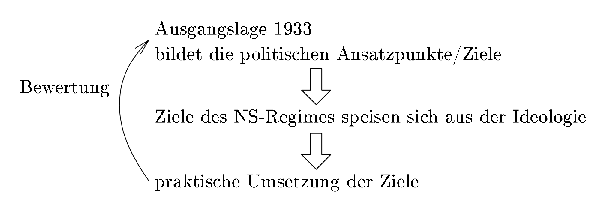
\includegraphics{bew-mass-ns.eps}
\caption{Bewertung der Wirksamkeit der Maßnahmen des NS-Regimes}
\label{pic:bew-mass-ns}
\end{figure}

Der Zustand der Weimarer Republik zu Anfang des Jahres 1933 bildete
die Ausgangslage für die Nationalsozialisten. Um deren Maßnahmen
hinsichtlich ihrer Wirksamkeit zu bewerten ist es zweckmäßig, zu
überprüfen, inwieweit sie Veränderungen gegenüber jener Ausgangslage
herbeiführten (siehe Abbildung \ref{pic:bew-mass-ns}) und wie die
Bevölkerung reagierte.

\begin{itemize}
\item wirtschaftliche Krise -- hohe Arbeitslosigkeit und Armut

\item Verhinderung wirtschaftlicher Erholung durch unfähige Demokraten
(\Nam{Brüning, Heinrich}{Brüning}s Deflationspolitik)

\item Wunsch nach
\begin{itemize}
\item Revision des \Ges{Vertrag von Versailles}{Vertrags von Versailles}

\item großdeutschem Reich -- Deutschland als militärische und
politische Großmacht

\item Verringerung der Arbeitslosigkeit
\end{itemize} 
\end{itemize}

%%%%%%%%%%%%%%%%%%%%%%%%%%%%%%%%%%%%%%%%%%%%%%%%%%%%%%%%%%%%%%%%%%%%%%

\subsection{Ziele der nationalsozialistischen Politik}

Aus dem vorhergehenden Abschnitt ergaben sich folgende Ansatzpunkte
für die Nationalsozialisten, um sich die Unterstützung der Bevölkerung
zu sichern:

\begin{itemize}
\item Wirtschaft
\begin{itemize}
\item Autarkie
\item Bekämpfung der Arbeitslosigkeit 
\end{itemize} 

\item Innenpolitik
\begin{itemize}
\item Ausschaltung der legalen Machtbasis
\item Zentralgewalt
\item Ausgrenzung der Nichtarier
\end{itemize}

\item Außenpolitik
\begin{itemize}
\item Revision des \Ges{Vertrag von Versailles}{Vertrags von Versailles}
\item Osterweiterung
\end{itemize}
\end{itemize}

Diese Ziele leiteten sich ebenfalls aus der Ideologie des
Nationalsozialismus ab, welche sich wiederum im \Ges{NSDAP,
Nationalsozialistische Deutsche Arbeiterpartei!Programm}{Programm der
NSDAP}\mycite{ProgNSDAP} niederschlug.

\endinput

\section{Innenpolitik}

\subsection*{NSDAP im Kabinett Hitler ab 30. Januar 1933}

\begin{description}
\item[\Nam{Hitler, Adolf}{Hitler}] Reichskanzler: Leitung der
Kabinettssitzungen, Bestimmung der politischen Richtlinien 

\item[\Nam{Frick, Wilhelm}{Frick}] Innenminister: verantwortlich für
die innere Sicherheit -- Vorbereitung und Durchführung von Gesetzen
und Notverordnungen (Zeitungs-, Versammlungs, Parteiverbot)

\item[\Nam{Göring, Hermann}{Göring}] Minister ohne Geschäftsbereich:
erhält das \ins{Reichskommissariat für das preußische
Innenministerium} -- Kontrolle über die preußische Polizei
\end{description}

%%%%%%%%%%%%%%%%%%%%%%%%%%%%%%%%%%%%%%%%%%%%%%%%%%%%%%%%%%%%%%%%%%%%%%

\subsection*[Maßnahmen Februar bis März 1933]{Maßnahmen Februar bis
März 1933\mycite[402]{gelbesGeschichts}}

Am \dat{1. Februar 1933} ließ \Nam{Hitler, Adolf}{Hitler} durch
\Nam{Hindenburg, Paul von}{Hindenburg} den \dat{Reichstag auflösen}.
Er begründete dieses Handeln damit, dass die Bildung einer
arbeitsfähigen Mehrheit im Parlament nicht möglich sei. Vorher hatte
er seine Scheinverhandlungen mit \Nam{Kaas, Ludwig}{Ludwig Kaas}
(Zentrum) scheitern lassen.

Danach begann der staatliche Terror, der die Ausschaltung
beziehungsweise Vernichtung der \jar{inneren} oder auch
\jar{Reichsfeinde} (Juden, gegnerische Politiker -- hauptsächlich KPD
und SPD) zum Ziele hatte. Gesetzliche Grundlage dafür war die
\dat{\ges{Reichstagsbrandverordnung} vom 28. Februar}. Diese führte
die \beg{Schutzhaft} ein; außerdem entstanden erste
Konzentrationslager.

Außerdem beeinflusste man im Hinblick auf die für \dat{März}
angesetzten \dat{Wahlen} die Bevölkerung durch Forcierung
propagandistischer Maßnahmen.

%%%%%%%%%%%%%%%%%%%%%%%%%%%%%%%%%%%%%%%%%%%%%%%%%%%%%%%%%%%%%%%%%%%%%%

\subsection*[Maßnahmen März 1933 bis August 1934]{Maßnahmen März 1933
bis August 1934\mycite[392\,--\,398]{gelbesGeschichts}}

Siehe dazu das Arbeitsblatt mit der Übersicht.

\endinput

\section{Wirtschaft}

\begin{aufgabe}
zu eingebunden -- siehe Hefter
\end{aufgabe}

\begin{itemize}
\item \jar{Rettung} der Bauern -- Ernährungs- und Lebensgrundlage
\item \jar{Rettung} der Arbeiter --
\textquote[{\mycite[139]{DeuzwDemuDikt}}]{umfassende[r] Angriff
gegen die Arbeitslosigkeit}
\item Autarkie $\Rightarrow$ Krieg
\end{itemize}

\begin{figure}
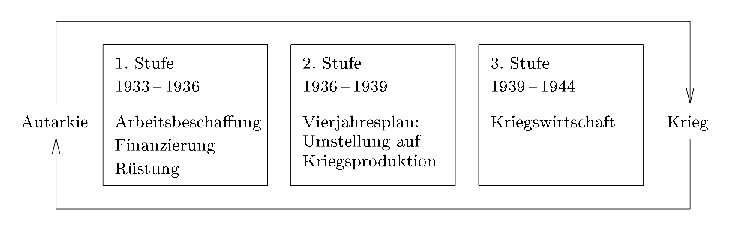
\includegraphics[width=\textwidth]{hit-stufpla.eps}
\caption{\Nam{Hitler, Adolf}{Hitler}s Stufenplan}
\label{pic:hit-stufpla}
\end{figure}

Diese Ziele wollte \Nam{Hitler, Adolf}{Hitler} mit seinem
\ges{Stufenplan} (siehe \ref{pic:hit-stufpla}) erreichen. Dessen erste
Stufe soll hier näher beleuchtet werden. \mar{Und die anderen?}

Die dargestellten Maßnahmen folgten der Politik des \emph{deficit
spending}\index{deficit spending}, welches durch den
Reichswirtschaftsminister und Reichsbankpräsidenten \Nam{Schacht,
Hjalmar}{Hjalmar Schacht} angeregt wurde. Er erfand auch das
sogenannte \emph{Mefo-Wechselsystem}\index{Mefo-Wechsel} zur
Finanzierung der Rüstungsaufträge. Nach diesem bezahlte nicht das
Deutsche Reich direkt selbst, sondern eine Scheinfirma, die \Ins{Mefo,
Metallurgische Forschungsgesellschaft}{Metallurgische
Forschungsgesellschaft} (Mefo) akzeptierte von der Industrie
ausgestellte Wechsel, die bis 1938 einzulösen waren. Die weiteren
Details sind hier unwichtig. Dieses System bot einige
Vorteile.\mar{Doch welche?}


\subsection{Erste Stufe: Wirtschafts- und
Sozialpolitik\mycite{LemoWirtsch}}
\mar{Wo sind die anderen?}

\subsubsection{wirtschaftliche Maßnahmen:}

\begin{itemize}
\item leichter Wirtschaftsaufschung 1933 durch die
Arbeitsbeschaffungsmaßnahmen der vorherigen Regierungen
\item Arbeitsbeschaffungsprogramme (Straßenbau: Autobahn, Bauwesen:
Wohnungsbau) steuerliche Anreize $\Rightarrow$ Senkung der
Arbeitslosigkeit
\item ab \dat{Juni 1935 Reichsarbeits- und Wehrdienst} $\Rightarrow$
Senkung der Arbeitslosigkeit
\item NS-Regime baut auf Privateigentum -- Interessenübereinstimmung
zwischen Großindustrie (Profitgier) und NS-Regime (forcierte
Kriegsvorbereitung)
\item schnelle Aufrüstung der modernen Industriezweige, beispielsweise
des Fahrzeugbaus
\item öffentliche Wirtschaftsforderung, vor allem durch
Rüstungsaufträge
\item Förderung der Landwirtschaft durch das
\dat{\ges{Reichserbhofgesetz} vom 29. September 1933}, das 
Hofteilung, Verkauf und Belastung mit Hypotheken verbot, dadurch aber
auch Neuinvestitionen stark behinderte.
\end{itemize}

\subsubsection{sozialpolitische Maßnahmen:}

\begin{itemize}
\item 1. Mai als staatlicher Feiertag bei voller Lohnfortzahlung
(1933 \ins{Feiertag der nationalen Arbeit}, ab 1934 \ins{Nationaler
Feiertag}) \index{1. Mai}
\item Gründung der Organisation \dat{\ins{Kraft durch Freude} im
November 1933} $\Rightarrow$ kulturelle und touristische
Freizeitbeschäftigungen für große Teile der Arbeiterschaft
\item Sofortmaßnahmen gegen Hunger, Armut und Verelendung, darunter
die Gründung des \dat{\Ins{Winterhilfswerk}{Winterhilfswerks}}
\end{itemize}

\endinput

\section{Außenpolitik}

Liest man \Nam{Hitler, Adolf}{Hitler}s Regierungserklärung vor dem
Reichstag vom 17. Mai 1933\mycite{HitlRegErklFrie} und seine Rede vor
der Reichswehrführung in Berlin vom 3. Februar des selben
Jahres\mycite{HitlRedRwfueh}, wird der zweischneidige Charakter seiner
Außenpolitik deutlich: Während er vor dem Reichstag von einer Heilung
der Wunden des Versailler Vertrages innerhalb der Grenzen der Verträge
und durch friedliche Auseinandersetzung mit \enquote{den Nationen}
spricht, fordert er vor der Reichswehr einen \enquote{Kampf gegen
Versailles} und \enquote{Sorge für die Bundesgenossen} unter
Verwendung kriegerischer Mittel.

Man erkennt also eine Verschleierungstaktik, die die eigentliche
Kriegsvorbereitung durch den scheinbaren Weg über Verträge verdecken
sollte. Zu den konkreten Maßnahmen siehe Tabelle
\ref{tab:massn-hitl-ausspol}. Für Karikaturen zu dem Thema siehe den
Hefter.

\begin{table}
\caption{Außenpolitische Maßnahmen Hitlers}
\label{tab:massn-hitl-ausspol}

\begin{tabularx}{\textwidth}{cXX}
\toprule
Jahr    & verschleiernd     & kriegsvorbereitend \\ 
\midrule
1933 & Konkordat mit dem Papst\index{Reichskonkordat} & \\
     & \multicolumn{2}{c}{Austritt aus dem
Völkerbund}\index{Völkerbund!Austritt des Deutschen Reiches}   \\

1934 & \ges{Deutsch-Polnischerr -Nichtangriffspakt} &  \\

1935 & Rückgliederung des Saarlands
(Volksabstimmung)\index{Saarland!Rückgliederung} &  \\
     & \ges{Flottenabkommen} mit Großbritannien &  \\

1936 & \Ins{Olympische Spiele!Deutschland}{Olympische Spiele} in
Deutschland & Rheinlandbesetzung \index{Rheinland!Besetzung} \\

1937 &  & Beitritt Italiens zum \ges{Antikominternpakt} -- \ins{Achse
Berlin\,--\,Rom\,--\,Tokio}\\

1938 &  & Anschluss Österreichs\index{Österreich!Anschluss an das
Deutsche Reich} \\

     &  & Sudetenkrise\index{Sudetenkrise} -- \ges{Münchener Abkommen} \\

1939 &  & \ges{Deutsch-Sowjetischer Nichtangriffspakt} mit geheimem
Zusatzprotokoll \index{Zusatzprotokoll} \\
\bottomrule
\end{tabularx}
\end{table}

\endinput

Hohohohohoho.

\section{Ausschaltung realer und vermeintlicher Gegner des NS-Regimes}
\label{sec:aussch-gegner}

\begin{aufgabe}
Erläutern Sie ideologische Grundlagen der Ausschaltung vermeintlicher
Gegner!

Beschreiben Sie die Umsetzung der Ideologie an den beiden
vermeintlichen Gegnergruppen! 

Bewerten sie die Maßnahmen auf der Basis demokratischer Politik- und
Moralvorstellungen!
\end{aufgabe}

\begin{aufgabe}
Arbeiten Sie aus dem Text die elemente des historischen Gesamtrahmen,
in dem sicher nationalsozialistische Massenmord entwickelten, heraus!

Der Autor behauptet, dass die Rolle Hitlers entscheindend für die
Judenverfolgung/-vernichtung war. Erarbeiten Sie die dazu gehörende
Argumentation anhand des Textes und die zu Grunde liegenden
ideologischen Ansätze!

\Nam{Friedländer, Saul}{Friedländer} nennt die ideologische
Radikalisierung des ausgehenden 19. Jahrhunderts als einen Faktor, der
in Kombination mit weiteren den Holocaust \enquote{vorbereitete}.
Überprüfen Sie diese Theorie der Radikalisierung innerhalb der
Maßnahmen des Regimes von 1933 bis 1945!
\end{aufgabe}


\begin{description}
\item[Grundlage:] Rassenideologie und Sozialdarwinismus
\index{Rassenideologie} \index{Sozialdarwinismus}
\item[Ziel:] Verhindern der Beeinträchtigung des \nat{deutschen
Volkskörpers} und Schaffung der \nat{reinen Rasse}
\end{description}

Die Höherentwicklung des deutschen Volkes (\nat{Herrenmensch}) wurde
laut Ideologie bedroht durch\footnote{Beide Bereiche greifen
ineinander. Die Trennung dient nur der Veranschaulichung.}\mar{Das ist
ein Fall von Scheinheiligkeit.}:

\begin{multicols}{2}
Unerwünschtes (\nat{lebensunwertes}) Leben:
\nat{schlechte Erbanlagen} bedrohen die Höherentwicklung des Volkes
sowie der Menschheit.

$\rightarrow$ \nat{Rassenhygiene}\\

\emph{Euthanasie}

\columnbreak

Juden und \nat{Art-}/\nat{Rassenfremde}: \nat{rassisch bedingte 
Verderbtheit der Juden als minderwertige Rasse}

$\rightarrow$ Rassenantisemitismus\\

\emph{\beg{Holocaust}}
\end{multicols}

%%%%%%%%%%%%%%%%%%%%%%%%%%%%%%%%%%%%%%%%%%%%%%%%%%%%%%%%%%%%%%%%%%%%%%

\subsection{Euthanasie}
\label{ssc:Euthanasie}
\index{Euthanasie}

\subsubsection{Gesetzliche Grundlagen}

\begin{chronik}
\item[14.\,7.\,1933] \ges{Gesetz zur Verhütung erbkranken Nachwuchses}:
Zwangssterilisierung von vermeintlich Erbranken -- circa 6\,000 Tote,
am meisten Frauen

\item[26.\,6.\,1935]
Ergänzung: Legalisierung des Schwangerschaftsabbruchs bei
diagnostizierter Erbkrankheit

\item[15.\,9.\,1935]
\ges{Gesetz zum Schutz des deutschen Blutes und der deutschen Ehre}:
siehe \ref{sss:nürnberger-ges}

\item[18.\,10.\,1935]
\ges{Ehegesundheitsgesetz}: Verbot von Eheschließungen mit geistig
Behinderten und Erbkranken

\item[1.\,9.\,1939]
\emph{Geheimer Führererlaß}: Ermächtigung zur Durchführung der
Euthanasie
\end{chronik}

\subsubsection{Aktion T4}
\index{Aktion T4}

\setlength{\parskip}{0mm}

Diese nach dem Krieg nach der Adresse -- Tiergartenstraße 4 -- der
Euthanasiezentrale in Berlin benannte Aktion beinhaltete die Umsetzung
des Euthanasiebefehls. Der daran beteiligte Personenkreis teilte
sich in vier Aufgabenbereiche:

Die \ins{Reichsarbeitsgemeinschaft Heil- und Pflegeanstalten} (Leiter:
\Nam{Heyde, Werner}{Werner Heyde} (medizinisch), \Nam{Bohne,
Gerhard}{Gerhard Bohne} (Verwaltung)) war für die Erfassung der Opfer
zuständig und verschickte zu diesem Zweck ab Ende 1939 Meldebögen, die
Auskunft über Art und Dauer der Krankheit und die Arbeitsfähigkeit
verlangten.

Die \ins{Gemeinnützige Stiftung für Anstaltspflege} (Leiter:
\Nam{Schneider, Willy}{Willy Schneider}) diente als offizieller
Arbeitgeber der etwa 400 T4-Mitarbeiter.

Die \ins{Zentralverrechnungsstelle Heil- und Pflegeanstalten} (Leiter:
\Nam{Kaufmann, Gustav a.}{Gustav A. Kaufmann}) wickelte die Kosten ab.

Die \ins{Gemeinnützige Krankentransport GmbH} (Leiter: \Nam{Vorberg,
Reinhold}{Reinhold Vorberg}) fuhr mit meist grauen Bussen die Opfer in
die Zwischen- beziehungsweise Tötungsanstalten.\\

\noindent Die Aktion T4 begann 1939 mit der Kindereuthanasie, dem
an mindestens 5\,000 erbkranken oder behinderte Kindern und
Säuglingen.  Wenig später wurden die Tötungen auf Erwachsene
ausgeweitet. Etwa 70\,000 geistig Behinderte, psychisch Kranke, mehr
als fünf Monate stationär Behandelte, Straftäter und
\nat{Fremdrassige} wurden dabei vergast.

Aufgrund von Protesten der Kirche, der Angehörigen und in der
Bevölkerung stellte man die Vergasungsaktionen 1941 offiziell ein. Da
man aber wegen des Luftkriegs gegen Deutschland immer mehr
Krankenhausplätze benötigte, begann nun die sogenannte \emph{Wilde
Euthanasie}\index{Wilde Euthanasie}: Etwa 30\,000 Menschen wurden
heimlich vergiftet oder zu Tode gehungert.

%%%%%%%%%%%%%%%%%%%%%%%%%%%%%%%%%%%%%%%%%%%%%%%%%%%%%%%%%%%%%%%%%%%%%%

\subsection{Die Verfolgung der Juden}
\label{ssc:juden-verf}
\index{Holocaust}
\index{Judenverfolgung}

% Breite der ersten Spalte
\newlength{\frstcoljud}
\settowidth{\frstcoljud}{Phase}
% Breite der übrigen Spalten
\newlength{\othcol}
\newlength{\othcolsum} % der ganze Rest
\setlength{\othcolsum}{\textwidth}
\addtolength{\othcolsum}{-\frstcoljud}
\setlength{\othcol}{0.25\othcolsum}
\addtolength{\othcol}{-2\tabcolsep}

\begin{tabular*}{\textwidth}{p{\frstcoljud}*{4}{p{\othcol}}}
Phase & \Rm{1} & \Rm{2} & \Rm{3} & \Rm{4} \\
      & 1933-35 & 1935-38 & 1938-41 & 1941-45 \\
      & Boykottaktio"-nen & Ausgrenzung durch Gesetz und Terror
      & Deportation & Endlösung
\end{tabular*}

\subsubsection{Boykottaktionen\mycite[135, 136]{GeschDrReich}}
\label{sss:boykott}
\index{Judenboykott}

\begin{chronik}
\item[1.\,--\,3.\,4.\,1933]
befristeter\footnote{Laut Frau Seipold schlug die Aktion fehl, da die
Bevölkerung aus Gewohnheit weiter bei Juden einkaufte.
\cite[135]{GeschDrReich} stellt das etwas anders beziehungsweise
differenzierter dar.} Boykott jüdischer Geschäfte\footnote{Diese
Aktion bildete das Ende der spontanen Gewalt gegen die jüdische
Bevölkerung. Was folgte, waren organisierte Verbrechen.}

\item[7.\,4.\,1933]
\ges{Gesetz zur Wiederherstellung des Berufsbeamtentums} (ein Art
staatlicher \emph{Arierparagraph}): Entlassung von
\nat{\beg{Nicht-Ariern}} aus dem öffentlichen Dienst

\item[7.\,4.\,1933]
Möglichkeit des Entzugs der Zulassung jüdischer Anwälte

\item[April 1933]
\ges{Gesetz gegen die Überfüllung der deutschen Schulen und
Hochschulen}: Verdrängung der Juden aus den
Bildungsanstalten\footnote{Der vollständige Ausschluß erfolgte 1938.}

\item[5.\,10.\,1933]
\ges{Schriftleitergesetz}: Verdrängung jüdischer Journalisten aus den
Redaktionen

\item[1934]
Pause von antijüdischen Gesetzen
\end{chronik}


\subsubsection[\dat{Nürnberger Gesetze 15. September 1935}]
{\dat{Nürnberger Gesetze 15. September 1935}
\mycite[417-419]{gelbesGeschichts}}
\label{sss:nürnberger-ges}
\index{Nürnberger Gesetze}

\paragraph{\ges{Reichsbürgergesetz}} 
Juden verloren alle politischen Bürgerrechte -- sie wurden statt
als \nat{Reichsbürger} nur noch als \nat{Staatsangehörige}
gesehen und somit aus der \emph{Volksgemeinschaft} ausgeschlossen.

\paragraph{\ges{Gesetz zum Schutz des deutschen Blutes und der
deutschen Ehre}}
Diese Gesetz verbot Juden

\begin{itemize}
\item Ehen und außereheliche Beziehungen mit \nat{Ariern}
\item die Beschäftigung \nat{arischer} Dienstmädchen unter 45
Jahren
\item das Hissen der \nat{Reichs- und Nationalflagge} und das
Zeigen der \nat{Reichsfarben}
\end{itemize}

In den Folgejahren wurden die Rechte der Juden durch Sondergesetze und
Verordnungen immer weiter eingeschränkt,
beispielsweise\footnote{In \cite[135-137]{GeschDrReich} ist dies
differenziert dargestellt.}:

\begin{itemize}
\item Entfernung aus Beamtenpositionen und Wegfall der Pensionen
\item Boykottierung jüdischer Geschäftsleute und Industrieller
\item Entzug jeglichen Rechtsschutzes
\item Ungültigmachung mit Juden geschlossener Verträge
\item Zutrittsverbot zu Hotels, Pensionen, kulturellen Einrichtungen
und Parks
\end{itemize}

\noindent $\Longrightarrow$ völlige Entrechtung und gesellschaftliche
Isolierung der Juden \\

Im Hinblick auf die \dat{Olympischen Spiele} in Deutschland reduzierte
man die Repressalien \dat{1936} wieder, nur um sie im folgenden Jahr
erneut zu forcieren.


\subsubsection{\dat{Reichspogromnacht 9./10. November 1938}}
\label{sss:pogromnacht}
\index{Reichspogromnacht}
\index{Reichskristallnacht}

Am \dat{7. November 1938} verübte \Nam{Grynspan, Herschel}{Herschel
Grynszpan} in Paris ein Attentat auf den dortigen Botschaftssekretär
\Nam{Rath, Ernst vom}{Ernst vom Rath}.  Dieses nahmen die
Nationalsozialisten in Deutschland zum Anlaß und Vorwand für
gewaltsame Aussshreitungen gegen Deutsche jüdischen Glaubens zwei Tage
später.

Im Zuge derer kam es zu Morden und Plünderungen, Synagogen, jüdische
Gebetshäuser, Friedhöfe, Geschäfte und Wohnungen wurden in Brand
gesteckt beziehungsweise zerstört. Der Name \emph{Reichskristallnacht}
rührt von den zahlreichen Fensterscheiben her, die in jener Nacht
zerschlagen wurden.

Die Folgen der \emph{Novemberpogrome} waren mindestens 1\,300 Tote,
mehr als 1\,400 zerstörte Synagogen, Verhaftungen und Deportationen
und weitere Verschlechterung der Lebensbedingungen für Juden. Für die
entstandenen Schäden von ungefähr 1,12 Milliarden Reichsmark mußten
die Opfer selbst aufkommen.

Mit dem endgültigen Verlust finanzieller Mittel wurde den Juden eine
eventuelle Ausreise aus noch weiter erschwert.


\subsubsection[Radikalisierung der Judenpolitik \dat{September
1939\,--\,1941}]
{Radikalisierung der Judenpolitik \dat{September
1939\,--\,1941}\mycite[209, 216]{GeschDrReich}\mycite[433,
434]{gelbesGeschichts}}
\label{sss:rad-jud-pol}

\paragraph{Deportationsmaßnahmen/-pläne} \index{Deportation}
Durch ihre Kriegserfolge angespornt, stellten die Nationalsozialisten
verschiedene Pläne, die Juden aus Europa zu verbannen, auf. Diese
wurde jedoch aufgrund der schieren Anzahl zu Deportierender nicht
umgesetzt: 

\begin{chronik}
\item[1939\,--\,1941]
Zwangsumsiedlung nach Polen, Zusammenfassung und Isolierung in
\beg{Ghettos} \index{Ghetto}

\item[1940]
(Sieg über Frankreich): \beg{Madagaskarplan} \index{Madagaskarplan}

\item[1941]
(Überfall auf die UdSSR): Umsiedlung nach Sibirien
\end{chronik}


\paragraph{Vorgehen der SS-Einsatztrup"-pen beim Überfall auf Polen}
während des Überfalls auf Polen führten die SS-Einsatztrup"-pen im
Schatten der Wehrmacht \nat{politische Säuberungen} durch: Mit dem
iel der Ausrottung der jüdischen Bevölkerung kam es zu
assenerschießungen und Massakern. In den ersten Kriegswochen starben
abei circa 5\,000 Menschen.

ußerdem wurde die Kennzeichnungspflicht für Juden eingeführt und
man pferchte sie in Ghettos zusammen, wo sie Zwangsarbeit für die
Rüstungsindustrie zu leisten hatten.

\paragraph{Vertreibung der Juden nach dem Polenfeldzug}
\index{Deportation}
Mit der Begründung, Wohnraum werde \nat{aus kriegswirtschaftlichen
Gründen dringend benötigt}, deportierte man die Juden in Lager
in der Gegend von Lublin und im \ort{Generalgouvernement}. Das geschah
zunächst Bewohnern des \ort{Gaus Warteland}, ein halbes Jahr später
denen aus \ort{Pommern}. Im \dat{Februar 1940} vertrieb man die
Juden aus der Gegend von \ort{Stettin} und im \dat{März 1940} aus
\ort{Schneidemühl} in Preußen.

\paragraph{Vorgehen gegen die jüdische Bevölkerung während des
Krieges gegen die Sowjetunion}
Mit dem Krieg gegen die UdSSR wurden die Tötungsaktionen des Überfalls
auf Polen fortgesetzt. Neben der Wehrmacht, die dabei in die
Machenschaften der SS integriert wurde, rekrutierte man nun auch Teile
der Bevölkerung als \nat{Reserve-Polizeibataillone} sowie verbündete
Truppen, vor allem aus Weißrußland und Rumänien.

Von den 4,7 Millionen sowjetischen Juden kamen so bis Ende 1942 2,2
Millionen zu Tode.


\subsubsection{Konzentrations- und Vernichtungslager -- Die
\nat{Endlösung der Judenfrage}}
\label{sss:konz-vern-endl}
\index{Konzentrationslager}
\index{Vernichtungslager}
\index{Endlösung}

\begin{chronik}
\item[Juni 1941]
Vergasungsanlagen für \ort{Auschwitz}, Einsatz ab Herbst als
Vernichtungslager\footnote{Nach \ort{Chełmno}, wo noch die sogenannten
\ort{Gaswagen} verwendet wurden\cite{WikChelmno}, war es damit das
zweite Vernichtungslager und sollte das größte derer werden.}

\item[31.\,7.\,1941] Anweisung an \Nam{Heydrich, Erwin}{Reinhard
Heydrich}, eine \nat{Endlösung der Judenfrage} zu finden

\item[20.\,1.\,1942]
\emph{Wannseekonferenz}:
\begin{itemize}
\item Organisation und Koordination der Deportation der europäischen
Juden
\item Beschluß, Juden in ganz Europa als Arbeistkräfte auszubeuten und
zu ermorden\footnote{Laut \cite{WikWannsee} war dieser Beschluß
faktisch schon gefaßt. Ich füge ihn hier ein, da sich kein anderer
Platz ergeben hat.}
\end{itemize}

\item[1942]
Errichtung weiterer Vernichtungslager in \ort{Bełżec}, \ort{Sobibór},
\ort{Treblinka} und \ort{Majdanek}
\end{chronik}

\endinput

\section[Widerstand]{Widerstand\mycite[116-125, 230-245]{GeschDrReich}}
\label{sec:widerstand}
\index{Widerstand gegen den Nationalsozialismus}

\begin{aufgabe}
Begründen Sie, warum trotz der Radikalität und Unmenschlichkeit des
Regimes der innerdeutsche Widerstand realtiv begrenzt blieb! 
\end{aufgabe}

\subsection[Definition]{Definition\mycite{WidDefschwieBeg}}

Es gibt immer wieder Debatten, wie der Begriff des Widerstands im
Nationalsozialismus zu definieren sei.\footnote{Selbst das hier
verwendete \cite{WidDefschwieBeg} weist hier Fehler in der logischen
Durchführung auf.} So schlug \Nam{Broszat, Martin}{Martin Broszat} in
den frühen Achtzigerjahren vor: \enquote{Wirksame Abwehr, Begrenzung,
Eindämmung der NS-Herrschaft oder ihres Anspruchs, gleichgültig von
welchen Motiven, Gründen und Kräften her.}

Es gab jedoch zahlreiche Kritik, die entgegesetzte, dass jene
Definition den Begriff zu weit fasse und schon bei \emph{Haltungen}
beginne, während man erst bei \emph{Handlungen} einsetzen
dürfe.\footnote{Ich bin anderer Ansicht. \enquote{Wirksame Abwehr,
Begrenzung, Eindämmung} sind für mich keine bloßen Haltungen.}
Weiterhin greift man die fehlende Berücksichtigung der Motive an.

Die Tendenz geht als hin zum Widerstand als
\textquote[\mycite{WidDefschwieBeg}]{Handeln, das auf grundsätzlicher
Ablehnung des Nationalsozialismus beruhte, das aus ethischen,
politischen, religiösen, soialen oder individuellen Motiven darauf
abzielte, zum Ende des Regimes beizutragen}.

Tabelle \ref{tab:widerst-def} gibt einen Überblick über verschiedene
Möglichkeiten der Definition.

% verfluchter Blocksatz
\begin{table}
\caption{Definitionen für \emph{Widerstand}\mycite{WidDefschwieBeg}}
\label{tab:widerst-def}

% Berechnung der Spaltenbreiten
\newlength{\colwidth}
\setlength{\colwidth}{0.33\textwidth}
\addtolength{\colwidth}{-2\tabcolsep}

\renewcommand*{\arraystretch}{1.5}

\begin{tabular*}{\textwidth}{*{3}{p{\colwidth}}}
\toprule

\multirow{2}{\colwidth}{\centering Widerstand im weitesten Sinn} &
\multicolumn{2}{c}{Widerstand im engeren Sinn} \\

\cmidrule{2-3}

&
kritische bis abweisende Haltung der Verweigerung und Selbstbehauptung
&
bewusste Anstrengung zur Änderung der Verhältnisse \\

\midrule

zusammenfassender Oberbegriff für gegen den Nationalsozialismus als
Ideologie und praktizierte Herrschaft gerichtete verschiedenartige
Einstellungen, Haltungen und Handlungen &
\emph{Verweigerung} als persönliche Abwehr von Herrschaftsanspruch und
Selbstbehauptung von Gruppen &
bewusster persönlicher Einsatz, verbunden mit einhergehenden
Gefährdungen \\

Umfasst also auch beispielsweise ins Exil geflohene, die kaum
Möglichkeit zur Einwirkung auf das nationalsozialistische Regime
hatten und die die sich weder durch Lockungen noch durch Zwang vom
Nationalsozialismus vereinnahmen ließen. &
\emph{Opposition} als Haltung grundsätzlicher Gegnerschaft gegen das
Unrechtsregime -- passiver Widerstand &
beispielsweise Planung des Sturzes der Diktatur (Attentate)
einhergehend mit der Errichtung einer neuen Gesellschaftsordnung --
aktiver Widerstand \\

\bottomrule 
\end{tabular*}
\end{table}

%%%%%%%%%%%%%%%%%%%%%%%%%%%%%%%%%%%%%%%%%%%%%%%%%%%%%%%%%%%%%%%%%%%%%%

\subsection{Gruppen}

Die deutschen Widerstandsgruppen kamen aus verschiedenen
gesellschaftlichen Schichten. Dabei ist der Mittelstand kaum
ernennenswert; dessen größte Teile waren dem \index{Hitler-Mythos}
Hitler-Mythos erlegen.

Etwas mehr, aber dennoch nur wenig, tat sich bei den Vertretern der
Industrie: Hier waren es hauptsächlich \Nam{Bosch, Robert}{Bosch} und
\Nam{Krupp von Bohlen und Halbach, Gustav}{Krupp}, die \Nam{Goerdeler,
Carl Friedrich}{Goerdeler} unterstützten und andere, die Kontakte zum
amerikanischen Geheimdienst unterhielten. Inwiefern man dabei jeweils
von \emph{Widerstand} sprechen kann, ist natürlich fragliche.

Schließlich formierten sich im politischen Lager zahlreiche locker
zusammengeschlossene Gruppen, die aber meist nur das gemeinsame Ziel
der Beseitigung des Regimes verband.

Alle waren allerdings der Meinung, dass die Befreiung vom
Nationalsozialismus von Deutschland selbst aus erfolgen müsse, da nur
so eine \emph{bedingungslose Kapitulation}, wie sie die Alliierten
forderten abgewendet und Souveränität und Verhandlungsfähigkeit
Deutschlands erhalten werden könnten.\mycite[191-193]{DeuzwDemuDikt}

Dabei waren die Widerstandsbewegungen im Ausland, beispielsweise die
\ins{R\'e{}sistance} in Frankreich und \index{Partisanen}
\ins{Partisanengruppen} in Polen, der Sowjetunion, Jugoslawien,
Griechenland und Italien, zum Teil viel reger und erfolgreicher als im
Reich selbst. Das lag daran, dass sich die politischen und geistigen
Strömung unter dem Eindruck eines gemeinsamen Besatzers zu einem
nationalen Befreiungskampf einten, während die Widerstandsgruppen in
Deutschland nur wenig zusammenarbeiteten, während die
Widerstandsgruppen in Deutschland nur wenig zusammenarbeiteten.

Anfangserfolge im Krieg hatten den \index{Hitler-Mythos} Hitler-Mythos
befeuert, Beamte und andere hatten einen Eid auf \Nam{Hitler,
Adolf}{Hitler} geschworen. Der Terror durch die \ins{Gestapo} und
scharfe Gesetze, die Kritik am Regime und Kontakte zum Ausland und zu
Ausländern im Inland verboten, taten ihr Übriges, um eine
Ablehnungshaltung der Bevölkerung gegenüber Widerständlern und
gewaltsamer Beseitigung der Obrigkeit zu schaffen.

Allerdings kehrte sich diese Haltung mit fortschreitendem
Kriegsverlauf immer weiter ins Gegenteil. Die Verschlechterung des
Zustands, insbesondere der Versorgungslage, ließ den Wunsch nach
baldigem Kriegsende immer größer werden; die unerwartete Kriegslage
verunsicherte das Regime, die Herrschaftsstruktur wurde löchrige,
sodass die Bevölkerung allmählich das Vertrauen verlor.

Im Folgenden sollen beispielhaft einige Gruppen mit ihren Motiven,
Zielen und Handlungen aufgeführt werden, die sich auch schon vor den
meisten Anderen gegen die nationalsozialistische Herrschaft gerichtet
hatte. Dabei werden sämtliche Grade von Kritik bis zum aktiven
Widerstand berücksichtigt.


\subsubsection[Kommunisten und Sozialdemokraten]{Kommunisten und
Sozialdemokraten\footnote{Die beiden Gruppen wirkten keineswegs von
Anfang an gemeinsam im Widerstand und auch später gab es teilweise
große Differenzen. So kämpften die Kommunisten zunächst ebenso gegen
die Sozialdemokraten und auch die Wahl der Mittel fiel unterschiedlich
aus: Während die Ersteren einigermaßen radikal und ohne Rücksicht auf
Verluste vorgingen, während die Anderen mehr Vorsicht walten ließen.}}
\index{Kommunismus}
\index{Sozialdemokratie}

Für deren Aktivitäten lagen natürlich ideologische Gründe vor.

\noindent Mittel:

\begin{itemize}
\item Flugblätter und Broschüren in großer Anzahl
\item Wandparolen
\item Demonstrationen
\item Fahnenhissen
\item Sprechchöre
\item Überzeugungsarbeit \enquote{von Mann zu Mann}
\item stille Verweigerung und
\textquote[{\mycite[120]{GeschDrReich}}]{öffentliche[s] Beharren auf
demokratischen und rechtsstaatlichen Idealen}
\item Milieubildung mit Nachbarschaftshilfe, Austausch von Meinungen,
Nachrichten und Spende von Trost
\item Fluchthilfe
\item Abhören ausländischer Sender
\item Zeitschriften und Publikationen, auch für das Ausland
\end{itemize}


\subsubsection{Kirchen}
\index{Widerstand!Kirchen}

Auch die Kirchen waren untereinander in ihrer Haltung gegenüber dem
Nationalsozialismus gespalten. Während die Katholiken sich zunächst
von \Nam{Hitler, Adolf}{Hitler} betören und täuschen ließen und später
eher seichte Mahnungen an das Regime richteten, wurde das anfängliche
Verlangen der Protestanten nach einem \nat{starken Mann} an der Spitze
des Staates befriedigt.

Allerdings vollzog sich mit der Zeit eine zunehmende Spaltung der
evangelischen Kirche in \Ins{Deutsche Christen}{Deutschen Christen}
als Anhänger des Nationalsozialismus und die \ins{Bekennende Kirche},
die ein entschlosseneres Unternehmen als die Katholiken an den Tag
legte.

Trotzdem muss man erkennen, dass weniger die Kirchen als Institutionen
selbst Widerstand leisteten, sondern eher christliche Einzelpersonen
-- besonders prominent sicherlich \Nam{Niemöller, Martin}{Martin
Niemöller} und \Nam{Bonhoeffer, Dietrich}{Dietrich Bonhoeffer} --
offen gegen den Nationalsozialismus vorgingen.\\

\noindent Kritikpunkte:

\begin{sloppypar}
\begin{itemize}
\item Kampf gegen Ordensgemeinschaften
(\nat{Klostersturm}\index{Klostersturm})
\item \textquote[{\mycite[121]{GeschDrReich}}]{\enquote{Pfaffenprozesse}
\index{Pfaffenprozesse} gegen Ordensgeistliche wegen angeblicher
Devisenschiebereien und Sittlichkeitsvergehen}
\item Eingriff des Staats in Kirchenangelegenheiten
\item Missachtung des \Ges{Reichskonkordat}{Reichskonkordats}
\item Rassenpolitik, Antisemitismus
\item Euthanasie
\item \nat{rassisch-völkische Weltanschauung}
\item Konzentrationslager
\item Willkür der \ins{Gestapo}
\item Missachtung christlicher Grundsätze
\end{itemize}
\end{sloppypar}

\noindent Mittel:

\begin{itemize}
\item Enzyklika \index{Enzyklika} \ges{Mit brennender Sorge}, geheim
vervielfältigt und verteilt
\item Eingaben\footnote{Diese waren eher zurückhaltender Art und
natürlich auch kaum erfolgreich.}
\item Reden von der Kanzel aus -- Predigten
\item \ins{Pfarrernotbund}
\item Untergrundarbeit
\end{itemize}


\subsubsection{Kreis um \Nam{Goerdeler, Carl Friedrich}{Carl Goerdeler}}

Hierzu gehörten hochrangige Militärs (beispielsweise \Nam{Beck,
Ludwig}{Generaloberst Ludwig Beck}), Wirtschaftsverantwortliche,
Industrielle, Gewerkschafter und andere vornehmlich konservative,
christliche und nationalliberale Bürger und Politiker. \\

\noindent Kritikpunkte:

\begin{itemize}
\item waghalsige Kredit-, Finanz- und Wirtschaftspolitik
\item Antisemitismus (negative Wirkung auf das Ansehen Deutschlands im
Ausland)
\item Entfernung des Denkmals für \Nam{Mendelssohn-Bartholdy,
Felix}{Felix Mendelssohn-Bartholdy} in Leipzig
\item Unterschätzung des Auslands
\item Kriegsbestrebungen
\end{itemize}

\noindent Ziele:

\begin{itemize}
\item Staatsstreich
\item Staats- und Gesellschaftsordnung auf Grundlage von
Rechtsstaatlichkeit, Moral, bürgerlichem Anstand und christlicher
Weltanschauung -- stark restaurativer Charakter
\item Kriegsende
\end{itemize}

\noindent Mittel:

\begin{itemize}
\item Kritik in Wirtschaftsgutachten für die Regierung
\item Werbung für Opposition gegen die Nationalsozialisten im Ausland
\item Knüpfung von Beziehungen zu Personen in verschiedensten
gesellschaftlichen Positionen
\item Einsatz des Militärs -- Verhandlungen mit hochrangigen
Offizieren
\end{itemize}


\subsubsection{Kreisauer Kreis\index{Kreisauer Kreis}}

Hier handelte es ich um eine Gruppe von Regimegegner
unterschiedlichster Profession, die sich auf dem Gut des \Nam{Moltke,
Helmuth James Graf von}{Helmuth James Graf von Moltke} in
\ort{Kreisau}, \ort{Niederschlesien}, zu Gesprächen traf. Führender
Kopf war neben dem Gutsbesitzer \Nam{Wartenburg, Peter Graf Yorck
von}{Peter Graf Yorck von Wartenburg}.

Bei dieser Gruppe muss man außerdem hervorheben, dass sie
hauptsächlich von den Verbrechen der Nationalsozialisten gegen Juden,
Kriegsgefangene und Bewohner der besetzten Gebiete zum Widerstand
angeregt wurden. Das war bei den bisher genannten Personen und
Körperschaften nicht primär der Fall.\\

\noindent Ziele\footnote{In diesem Abschnitt werden zahlreiche
Wortkombinationen verwendet, wie sie genau so in
\cite[236-238]{GeschDrReich} zu finden sind. Ich verzichte auf
ständige Anführungszeichen und Partikulärnachweise.}:

\begin{itemize}
\item Überwindung des Nationalsozialismus, des Machtstaats und des
Rassendenkens

\item Neuordnung und Neuorientierung von Staat und Gesellschaft
\begin{itemize}
\item Wiederherstellung eines humanen Rechtsstaats
\item Garantie von Glaubens- und Gewissensfreiheit
\item Recht auf Arbeit und Eigentum
\item Selbstbestimmung und Verantwortlichkeit statt Befehl und
Gehorsam
\item politische Verantwortung und Mitwirkung jedes Einzelnen statt
Diktatur und Unterwerfung
\item Gründung einer Völkergemeinschaft im Geiste internationaler
Toleranz
\end{itemize}

\item Bestrafung der nationalsozialistischen Verbrecher
\end{itemize}

\noindent Prinzipien:

\begin{itemize}
\item Humanität
\item christliche Ethik
\item Gerechtigkeit
\item Ablehnung von Gewalt\footnote{Hiermit ist hauptsächlich die
Ablehung eines gewaltsamen Sturzes des Regimes und einer Ermordung
\Nam{Hitler, Adolf}{Hitlers} gemeint. \Nam{Moltke, Helmuth James Graf
von}{Moltke} befürchtete nämlich, dass ein solches Vorgehen nach dem
Umsturz ähnlich der \emph{Dolchstoßlegende}\index{Dolchstoßlegende}
propagandistisch ausgeschlachtet würde.}
\end{itemize}


\subsubsection{Weitere}

Mit den genannten Gruppen ist ein großer Teil des Spektrums der Motive
und Ziele von Widerstandsgruppen abgedeckt. Für weitere Informationen,
insbesondere über die Attentate auf \Nam{Hitler, Adolf}{Hitler} und
über studentischen Widerstand wie den der \Ins{Weiße Rose}{Weißen
Rose} siehe auch \cite[239-245]{GeschDrReich}.

\endinput


\endinput
